\documentclass{article}
\usepackage[letterpaper]{geometry}
\usepackage[usenames,dvipsnames,svgnames,table]{xcolor}
\usepackage{natbib,setspace,lineno,amsmath,graphicx}

\newcommand{\dc}{{\color{red} \it (Data Collection)}}
\newcommand{\dr}{{\color{red} \it (Data Reuse)}}
\newcommand{\du}{{\color{red} \it (Data Use)}}
\newcommand{\SabLatin}{{\it Anoplopoma fimbria}}

\newcommand{\sj}[1]{{\color{red}\mbox{}\marginpar{\raggedleft\hspace{0pt}*} SJ: #1}}

% ToDo: Break into the two major sections: avoidance and stock assessment. Each of these could be a separate PhD. Then, develop avoidance deeply for 802.

% In future, develop stock assessment deeply, this will give an off the shelf proposal outline for stock assessment. This might encourage a switch, or give a PostDoc proposal.


\title{Data-oriented approaches for avoiding bycatch in BC's groundfish fisheries.}
\author{Samuel Johnson}

\begin{document}
\doublespace

\maketitle

\newpage

{ \small
\tableofcontents
}

\newpage
\section{Introduction}\label{sec:intro}

With the emergence of eco-certification groups like SeaChoice and Seafood Watch, consumers are able to directly place market pressure on fisheries with poor records of sustainable management and biodiversity preservation \citep{Pelc201556}. One way that these groups evaluate biodiversity preservation is by studying the fishing induced mortality rates of target and non-target species. There are two main sources of mortality for target and non-target species: 
\begin{enumerate}
  \item[(i)] bycatch, which is broadly defined as interaction between non-target species and fishing gear; and
  \item[(ii)] discarding, which is the return of unlanded catch to the water.
\end{enumerate}
Both sources impact future spawning stock abundance, which in turn affects the long-term economic and ecological sustainability of the fishery.

Bycatch and discard rates are a concern of marine fisheries worldwide \citep{hall2005managing}. The reduction of mortality induced by discarding and bycatch is an increasingly active area of academic, public and private research, as shown in Figure \ref{fig:WoSPubRep} \citep{saila1983importance,pascoe1997bycatch,FAO1997,gilman2006fleet,davies2009defining}.  Global estimates of mortality due to bycatch and discarding vary a lot depending on definitions of bycatch and methods for estimation, which is illustrated in the following three examples. First, by considering bycatch as a function of landings, \citet{AlversonEtal1994} estimate between 17.9 and 38.5 million metric tonnes per year in the late 1980s. Second, by considering bycatch as a function of a fishery - defined as a combination of gear, stock and area - \citet{kelleher2005discards} estimated that annual bycatch was most probably around 6.8 million metric tonnes in the late 1990s. Finally, by defining bycatch as any removals which are unused or from an unmanaged species, \citet{davies2009defining} estimate that bycatch accounted for $40.4\%$ of global marine catches in the early 2000s.

Approaches to bycatch reduction generally fit into one or more of the following three categories: (i) technological; (ii) regulatory; and (iii) social \citep{hall2005managing}. Technological approaches address issues of selectivity, deterrence and avoidance through gear modifications, like bycatch reduction devices (BRDs) and communication. Examples of regulatory approaches include catch and discarding limits enacted through quota systems, bans on discarding and enforced landing and usage of bycatch. Social approaches include techniques such as economic analyses to make benefits and costs of bycatch explicit and institution building from the bottom up to encourage self regulation at the level of the fishery.

Each of the three approaches outlined above can have perverse side effects which ultimately increase the volume of removals taken as bycatch, suggesting that no single approach is best and a combination of all three may be required. Regulatory approaches on output, such as placing individual or fleet quota restrictions on target and bycatch species can encourage discarding behaviour known as high-grading if not sufficiently monitored \citep{branch2006replacing,Abbott2009195}. Avoidance and gear modification can reduce the catch of target species but sometimes also lead to increased effort and higher absolute bycatch mortality. Similarly, social approaches can carry the weight of the majority in a fishery, but this is a double edged sword which may lead to organised resistance against bycatch reduction efforts.

\sj{The following paragraph doesn't hang together very well. The main idea should be the negative space left by an absence of data-based methods, but there are sentences about gear-based reduction methods.}
Quantitative analysis of commercial data is conspicuously absent from bycatch reduction approaches, aside from uncommon ad-hoc uses in fleet communication programmes \citep{gilman2006fleet}. This absence suggests opportunities for the study of data-based methods. For example, \citet{hall2005managing} recommended gear modifications as the most efficient solution, estimating a reduction of 25\% to 64\% of yearly bycatch induced mortality if experimental techniques are replicated at a global scale. The improvements estimated by \citet{hall2005managing} suggest that gear based techniques are under-adopted for some reason, perhaps due to costs or the regulatory environment.

Fisheries data are usually collected for regulatory and stock assesment applications and are often left under utilised; sometimes the data isn't even being used for their intended purpose. We aim to investigate possible data-based techniques for avoidance of bycatch species, finding secondary uses for commercial fishing data where possible and creating new streams of data where appropriate. Specifically, we intend to answer the question: \textbf{How can data be used to help avoid non-target species in a multi-species fishery?} Any resulting techniques would complement existing regulatory structures, and would be developed in partnership with harvesters. 

\subsection{Discarding of Sablefish in the BC Integrated Groundfish Trawl Fishery} \label{sec:BCGTF}

The BC integrated groundfish trawl fishery (GTF) is a multispecies fishery operating year round along the entire coast of BC \citep{PRIFMP2010}. The BC GTF is a prime candidate for the study and experimentation of data-based methods of bycatch avoidance, due to the currently implemented social and regulatory approaches to bycatch reduction and limited options for techonological approaches. The GTF was originally integrated in order reflect the realities of catch composition and reduce discard induced mortality of commercial species discarded as bycatch when targeting other species. Quota is assigned to harvesters for every commercial and bycatch species they will encounter and is calculated on caught weight rather than landed weight. Fishing events are monitored by a 100\% at sea observer programme (ASOP), in which on-board independent observers monitor and record catch weight, composition and discarding and report their observations to Fisheries and Oceans, Canada (DFO).

Sablefish (\SabLatin) are a commercial species of groundfish whose migratory habitat intersects the area fished by the GTF and are considered a bycatch species by GTF harvesters. Sablefish are targeted by a separate, directed fishery and migrate across the GTF fishing banks during their juvenile life stage. Quota is therefore distributed to GTF quota holders for marketable sized (greater than 55cm) sablefish, which amounts to approximately 10\% of the total allowable catch (TAC) for sablefish acrosss all BC fisheries \citep{PRIFMP2010}. Due to the low amount of quota available, harvesters will sometimes choose to discard marketable sablefish with a discard mortality rate applied rather than to retain them, despite their high value.

Sablefish stocks are in decline across the entire west coast of North America \citep{hanselman2009assessment,stewart2011status}. Whether this decline is due to interception of sablefish in other fisheries during migration or something else remains unclear. In fact, discarding of marketable sized sablefish is of low concern in the GTF amounting to around 100t per year, with an estimated 25t per year of discard induced mortality. The value of landed sablefish incentivises retention of marketable pieces and the ASOP disincentivises high-grading behaviour. Moreover, marketable discarding accounts for around 20\% of the discards, with the remainder made up by unmarketable discarding.

Conversely, juvenile sablefish discards in the BC GTF are of growing concern, with around 300t of juvenile fish discarded each year. While the discards are not disincentivised by quota, the economic value of the stock and the possible effect of juvenile discarding on future spawning and landings provides incentive for stakeholders to halt the decline. Further, the 100\% ASOP provides fully audited, trustworthy data for analysis. With the availability of rare, trustworthy data and the concerns surrounding continued juvenile discarding, we see the GTF as a good focus for our study on data-oriented approaches.

This research aims to provide answers the following questions:
\begin{enumerate}
  \item {\it What, if any, are the predictors for the presence of juvenile sablefish?} \label{Q:predictors}
  \item {\it How can we improve the spatial and temporal resolution of movement data without exploding the cost?}
  \item {\it How can fleet communication be used to juvenile sablefish? What aspects can be automated?}
  \item {\it What general equipment can be designed to integrate the movement detection and fleet communication into a real-time feedback system to facilitate harvester avoidance of bycatch species?}
  \item {\it What are the estimated costs associated with sablefish bycatch in the GTF now, and what is the expected economic benefit from sablefish avoidance strategies?}
\end{enumerate}


\section{Can bycatch be predicted?}\label{sec:predBycatch}

\subsection{Background}

\sj{Is this talking about social and ecological drivers, or about predictive capabilities of data? Work it out.}

Beginning in 1997, The GTF has had an at-sea observer programme (ASOP) with 100\% coverage of the fishery. This means that on every fishing trip an observer records details of the entire catch, including species composition, discarded catch, trawl location and time. The ASOP has produced a large volume highly granular data while it has been in operation: between 1997 and 2006 there were a total of $6471$ fishing trips in the GTF and a total of $128,466$ trawling events, all of which were recorded in the PacHarvTrawl database at the Pacific Biological Station.

Ecological and social factors in discarding and bycatch are suggested by the ASOP data from the GTF. First, changes in bycatch rates of juvenile sablefish in the GTF appear to have a seasonal pattern, with higher than average bycatch in January of each year (Figure \ref{fig:bycatchTS}), commensurate with the seasonal migration and spawning habits of sablefish \citep{beamish1988resident}. This suggests an ecological factor at play in bycatch incidence. Second, there is a slight bias towards a subset of skippers in the discarding behaviour. Those skippers who discard more than 1t of juvenile sablefish in a single event are responsible for about 10\% more discarding than fishing; this might be noise rather than signal, but also might be suggestive of a social driver.

In this chapter, we aim to answer the question: \textbf{``Can we predict sablefish bycatch in the GTF with the data collected by the ASOP?''}. Given the unique, granular data we have access to here in the BC GTF, we are optimistic that we can. Of interest to us is the question of whether fishing events with high amounts of discards were predictable based on the previous fishing events on the trip. If such events are evident, social drivers might be present: skippers could see the bycatch in the future, but somehow the incentive structure either drove them towards it or failed to drive them away. Our question therefore becomes more specific: ``What are the covariates in the GTF ASOP data which best predict bycatch and discarding on a per-event and per-trip basis?''

\subsection{Methods}

To determine the ability of GTF ASOP data to predict sablefish discarding, we will employ a Bayesian network \citep{nagarajan2013bayesian} to estimate the amount of discarding given certain ecological and social conditions. Discarding for a single event and total discarding for a trip will be response variables in the network. 

Bayesian networks allow a hierarchical modeling approach which reflects the indirect effect that covariates have on responses, as opposed to a linear or additive model which assumes that covariates affect responses directly. Bayesian networks consist of two parts: a directed acyclic graph (DAG) and a set of conditional distributions. Nodes in the graph represent predictors or response variables, and arcs represent hierarchical dependencies.

Bayesian networks have two advantages over traditional hierarchical models. First, the graphical structure of the model allows for expert input on the model without the need for statistical expertise. Second, complete specification of all parameters of each covariate distribution is unncessary, significantly reducing the parameter space of the model due to conditional independence of covariates implied by the model structure. These advantages allow for easy input from stakeholders now, and computational advantage for updating the model later.

We will use two network topologies for comparison of performance; initially, a network topology based on our best knowledge will be used and is shown in Figure \ref{fig:BN}, but this will be updated with input from harvesters in Summer, 2015. These topologies will imply conditional dependence among covariates, the strength of which can be estimate from data. The next step in constructing the BN is to thoroughly investigate the conditional sample distributions and choose conditional distributions for the population. Finally, some of the continuous variables may have to be discretised in order to accomodate the data structure.

Once the network structure and conditional distributions are chosen, the model will be fit to a training sample of data using maximum likelihood estimates from generalised additive models at each node. Those nodes with parents will condition their distributions on the value of the parent nodes, while those without parents will be conditioned upon a prior distribution if necessary. A Gibbs sampling Markov chain Monte-Carlo technique will then be used to query the network on the remaining test sample of the data to test the inferential performance of the model.

The final stage of the model testing is to run a sensitivity analyses and cross validations, to test the robustness of the model to different network structures and different training-testing samples of the data. Both the harvester network and our initial network will be tested, using two sets of predictors: only ecological, and both social and ecological. Model performance will be measured for all four treatments by analysing the residuals between predictions and observations on historical data, and using a suitable posterior comparison technique.


\subsection{Expected Results}

We expect to produce a robust Bayesian network fit to 15 years of ASOP data from the BC GTF. The network will help us answer the question of whether prediction is possible. The measure of success will be the variance inherent in our posterior estimates given by the network when compared to test data, or future data coming down the line.

\subsection{Challenges and Proposed Solutions}

\subsubsection*{Conditional Distributions}

There are two foreseeable challenges with distributions at each node. First, fitting an hybrid BN to this set of data requires use of non-Gaussian distributions due to the high number of zeroes in distributions of otherwise positive data. This makes fitting the network to data a more complicated procedure and introduces some subjectivity into the model selection. Second, the distributions which are chosen based on the samples in the data may be inappropriate for the underlying population distribution. This could lead to overfitting of the data and provide inaccurate inferences.

The most obvious solution to both of these problems is extensive sensitivity and exploratory analyses of the model and the data. Sensitivity to chosen distributions can be tested, and among those distributions tested should be zero-inflated or hurdle distributions to account for zero-inflated data. Parsimony should be the guiding factor for conditional distribution choice, to avoid overfitting and subjectivity. Furthermore, exploratory analyses can help identify those cases where accounting for zero inflation will allow a transformation from non-Gaussian to Gaussian models, simplifying the fitting due to available software for Gaussian-Discrete hybrid networks \citep{nagarajan2013bayesian}.

\subsubsection*{Model performance}

It might turn out that the model performance may be terrible, or hinge on an effect which essentially undermines the predictive power. In the first case, posterior distributions produced by queries to the model may have so much variance that the actual predictive power is close to zero. In this case, more data may be required, or perhaps the answer to our question is that we cannot predict discarding with this model.

For the second case, consider the year effect on discarding. A year effect is impossible to rely upon in future predictions of discarding, at least at the beginning of the year. Thus, the year covariate should be the subject of sensitivity analyses to determine the extent of the year effect. An option for accounting for recent effects may be instead to use the most recent quarter as a prior on a time varying effect - this requires deeper thought than we've given it so far.


\section{What is the cost of sablefish discarding?}\label{sec:economics}
    
\subsection{Background}

Not every sablefish survives at-sea discarding. Discarded marketable sablefish in the GTF are assumed to die at a rate dependent on the duration of the trawling event, with the dead discarded fish removed from the harvester's quota. However, harvester quota is not affected by the discarding of unmarketable sablefish, but it stands to reason that the survival of the fish is affected in a similar way. Discard induced mortality of juveniles is therefore an external cost to the sablefish fishery, due to the subsequent loss of landings and spawning potential.

The extent of the cost of discard induced mortality to the fishery is unquantified. We aim to quantify this impact both ecologically and economically by using a bio-economic model. The model will then inform a prospective analysis of future landings and stock size under different discarding scenarios.

\subsection{Methods}

In order to quantify the ecological and economic impact of discard induced mortality, we propose the use of a bio-economic model of the fishery. Initially, population dynamics will follow a production model, similar to a Schaefer model \citep{schaefer1957some}, with recruitment to the fishery affected by juvenile discard-induced mortality as a lagged effect to account for maturation rates. The population model will be fit to historic commercial and survey data for parameter estimation. After fitting the population dynamics model, we simulate future activity using different harvest rules and discarding behaviour. For each scenario a net present value of the fishery will be computed using a discounted cash flow analysis based on the value of landed catch.

Further additions to the model might include the cost in person-hours of sorting and discarding unmarketable catch in other fisheries and the inclusion of non-market values such as existence value and eco-system services provided by the stock.

\subsection{Expected Results:} 

While the status quo might be a potentially Pareto efficient situation, we expect the outcome of a reduction in juvenile mortality to be favourable to the status quo.

\subsection{Expected Challenges and Proposed Solutions}

\subsubsection*{Variability}

One challenge could be an unmanageable amount of variability in estimates which arise from the modeling. This variability could be caused by improper specification of the parameters or some fundamental error in the choice of dynamic model. One glaring example is how to properly include the effect on recruitment of discard induced mortality of juveniles.

The solution to a problem in parameter variability depends on the exact nature of the problem. For model selection issues, a model selection criterion would probably suffice, such as AIC, BIC or reversible jump MCMC \citep{gelman2014bayesian}. 

\subsubsection*{Market Failures}

Another challenge is the proper identification of market failures, specifically external costs. Also, once the source of such costs are identified, finding explicit data to help estimate them might be troublesome. In these cases, the solution will be to take a bounding approach to the model and replace variables with point estimates or prior distributions.


\section{Can the spatial and temporal resolution of movement data be improved without exploding the cost?}\label{sec:PowSim}

\subsection{Background}

Movement of animals is characterised by multiple movement modes at multiple spatio-temporal scales \citep{nathan2008movement,fryxell2008multiple}. At the fine scale, animals are often either resting or foraging; at the coarse scale either cycling around feeding locations in a home range or migrating between areas. Some studies of movement data account for mode changes by allowing for each time step between data points to be described by a single Fundamental Movement Element (FME) with some constant, average rate. However, depending on the resolution of the data, it might instead be more realistic to assume that a composite of movement modes - for instance: swimming slowly, swimming fast, foraging and resting - were active in the space of a single time step. 

A mismatch of spatio-temporal resolution and the rate at which movement modes are changing can be accounted for within movement models in two ways. First, the time resolution of sampling can be refined so that switching of movement modes happens less often than a single time step. Second, we can use composite collections of FMEs called Canonical Activity Modes (CAMs) \citep{fryxell2008multiple}. CAMs are used as a distribution of FMEs over a given time scale , and while a single CAM is unlikely to account for all of an individual's time, it is reasonable to assume that the correct combination of CAMs can account for most if their time. \sj{Can we include some more info from \citet{nathan2008movement} here, specifically the influence of internal state and external factors on movement? Also, there seem to be two ideas here: one about increasing resolution, and one about CAMs.}

Sablefish are tagged using passive tags in nearshore inlet surveys, stratified random surveys and the traditional \sj{check} surveys in each year. An average of \sj{figure} tags are released each year, and an average of \sj{figure} are recovered by commercial fisheries and surveys with an average of \sj{figure} days at liberty. The data generated by these tagging programmes is used to estimate abundance in different areas and movement probabilities between areas. However, there are two drawbacks to the current tagging data and its use. First, the tagging data is quite coarse both spatially and temporally, with data points separated by several hundred kilometres and several hundred days \sj{give concrete data here, this fits with the first two sentences}; moreover, tagged sablefish often provide at most two data points because detection is usually associated with fishing mortality. Second, the models that are used to analyse the data take individual based data and aggregate it into population based behaviour. \sj{This might be a better second paragraph, to introduce the Challenge. Then the current 2nd par can perhaps form part of the methods (Action)}

This chapter aims to answer the question `How can we increase the spatio-temporal resolution of sablefish movement data without exploding the cost?' Specifically, we investigate the efficacy of replacing traditional tags with acoustic or archival tags, and accounting for multiple movement modes when analysing movement data. Given the increased cost of active tags and detection gear, a power analysis is performed to compute the required sample size of tagged fish to match or improve upon the status quo.


\subsection{Methods}

To generate data for the power analysis we use an individual based model of tagged sablefish and trawl vessels on the BC coast. The model is a combination of a Discrete Event Simulation (DEVS) for the fishing vessels and a discretised Stochastic Differential Equation (SDE) for tagged fish.

\subsubsection*{Fish movement}

Fish move according to a depth preference by following bathymetric gradients; process error in the form of Brownian motion is added for variability in fish behaviour. Explicitly, for a given fish $f$ let $p_f(t) = (x_f(t), y_f(t))$ be the position in latitude and longitude of $f$ at time $t$. If $z(x,y)$ is the depth of the sea-floor at the coordinates $(x,y)$ then the fish $f$ moves according the the SDE
\begin{equation}\label{eq:SDE}
\frac{dp}{dt} = \omega \cdot \left( - \frac{\partial z}{\partial x}, - \frac{\partial z}{\partial y} \right) + (\epsilon_x, \epsilon_y). 
\end{equation}
In \eqref{eq:SDE}, the partial derivatives of $z$ are the downhill bathymetric gradients, representing a preference of sablefish for deepwater habitats. The multiplicative weight $\omega$ rescales the jumps so that sablefish move at approximately 0.6 body lengths per second, as found for pacific cod by \citet{hanna2008temperature} - analogous data for sablefish was unable to be found in the literature. Finally, the 2 dimensional process error term $(\epsilon_x, \epsilon_y) \sim \mathcal{N}(0, \sigma^2)$ introduces stochasticity into jumps to account for latent effects uncaptured by the habitat preference function; $\sigma^2$ is chosen sufficiently small to keep movement speeds realistic.

Multiple movement modes will be included in further iterations of the model, most likely these will take the form of different types of potential functions. These potential functions will add to \eqref{eq:SDE} by adding a small vector towards a certain point or an auto-correlated direction preference. By using such methods to add a small bias to the stochasticity, home ranging or migration patterns can be included in such a way that the simulated movement is still fairly natural.

\subsubsection*{Trawler movement}

Under any tagging programme trawlers can only detect the fish while fishing gear is deployed. Because time between fishing events is uninteresting from the point of view of a fish, only discrete fishing events need to be simulated. The simulation of boats therefore is done under a discrete event simulation (DEVS) framework. \sj{citation}

Our DEVS framework consists of a future event list (FEL), a clock and a state array for each boat. Initially, a time stamp for the first fishing event is picked at random and the event is placed on the FEL, along with details such as event duration and location. Events on the FEL are processed in the following way:
\begin{enumerate}
  \item Forward clock to time stamp of next event. \label{list:nextEvent}
    \begin{itemize}
      \item If docking reset trip duration counter, create new fishing event, go to \ref{list:nextEvent}.
    \end{itemize}
  \item Update boat states for event duration: location, fishing or docked, total trip duration.
  \item Check trip duration:
  \begin{itemize}
    \item if above threshold, create docking event with random layover time;
    \item if still under treshold, randomly choose interfishing time, create new fishing event.
  \end{itemize}
  \item End event processing, go to \ref{list:nextEvent}.
\end{enumerate}
This processing algorithm allows us to ignore any non-fishing time for each boat and gains significant computational advantage in the simluation stage. Interfishing times, layover times and fishing location choices are chosen from distributions with parameters based on historic commercial data.

\subsubsection*{Detections}

Fish and trawlers are simulated in a pre-processing stage to generate system states for every time step. Time steps are 1 hour intervals, while trawl events are between 30 minutes and 3 hours long. To overcome this difference in time-scales, detections will be simulated in a case by case basis.

During each fishing event the model checks if any fish are within a certain threshold distance of the fishing location, any event for which a fish is close enough is defined as an {\it opportunity for detection}. Each opportunity for detection triggers a secondary simulation on a more refined spatio-temporal scale. This nested simulation allows us to record how much time a fish spends within a detection radius of the fishing gear, and will also facilitate simulation of fishing mortality. 

Detections will be simulated based on the tagging programme. Detections of acoustic tags will depend on frequency of pings, time spent in proximity to detection gear and a detection efficiency. Detections of archival or traditional tags will depend on fishing mortality. Detection rates will be our first level of power analysis, allowing a ranking of performance among tagging programmes with differing sample sizes.

\subsubsection*{Estimation and Validation}

\sj{Include adehabitat stuff}

Finally, we will use simulated detection data for all types of programmes to estimate movement behaviour of the simulated fish. This will involve several models, from simple markovian style models \citep{mcgarvey2002estimating} to state-space models which include several movement modes \citep{fryxell2008multiple}. The estimation success will be used to rank tagging programmes based on the speed at which they facilitate unbiased learning.


\subsection{Expected Results}

We expect to build a fairly general and adaptable individual based simulation model, validated against the early 1990's fixed location sablefish survey data. The model will allow us to compare the benefits of several tagging experiments using traditional, acuoustic and archival tags. This comparison will also enable a power analysis to estimate the required sample size in a given programme, helping identify trade-offs between tag cost and the value of information.

\subsection{Expected Challenges and Proposed Solutions}

\subsubsection*{Inconvenient Bathymetry}

In order to encourage the fish to swim towards the continental shelf the SDE for fish movement relies on bathymetry. However, in some cases the bathymetry is quite inconvenient for this simple approach and the `downhill' direction is in fact away from the realistic average direction of migration. For instance, in all four inlets the water is deeper than the water on the continental shelf; in this case, the majority of fish will congregate in one area and any that make it out of the inlets owe their success solely to the brownian process error.

One possible solution to the problem is to change \eqref{eq:SDE} to include $\rho_q$ like so:
\[
\frac{dp}{dt} = \omega \cdot \left( - \frac{\partial z}{\partial x}, - \frac{\partial z}{\partial y} \right) + (\epsilon_x, \epsilon_y) + \omega' \rho_{q} ( x(t), y(t) ),
\]
where $\rho_q$ is defined as
\[
  \rho_q ( x(t), y(t) ) = (x_q, y_q) - (x(t), y(t) ).
\]
The function $\rho_q$ is called a potential function, as it in effect sets up a potential difference between the location of the fish at time $t$ and the point $q = (x_q, y_q)$. In the case of the inlets having deeper water than the continental shelf, setting $q$ out towards the changes the mean direction of travel towards the open ocean, overcoming inconvenient bathymetry without affecting the random component of travel. The weight constant $\omega'$ tunes the jump size to realistic proportions, but can also be used to switch the potential on and off based on the location of the fish. For instance, when the fish overcome the inconvenient bathymetry and are on the continental shelf, we can set $\omega' = 0$ and allow the bathymetry to drive the movement.

\subsubsection*{Realism}

Because of the bathymetric effect on the movement directions, fish will always swim to deeper water. While this may be a realistic behaviour while migrating, sablefish normally stop at the continental slope, with only a small number of individuals recruiting to seamount fisheries farther offshore. The currently proposed SDE doesn't reflect this behaviour, and under this model all individuals will eventually travel unrealistically far. 

The solution in this case will be similar to the inconvenient bathymetry. Possibilities include adding potential functions to simulate home ranging behaviour and setting weights to zero to remove components of the mean direction of travel.

\subsubsection*{Sample size effect is quite variable}

The effect of sample size on reducing variance in habitat detection varies a lot with the population in early iterations of the model. Sample sizes of $N = 10,~25,~50,~100,~250$ tagged fish in each inlet were tested 25 times each. The performance of each sample size is shown with 95\% confidence regions in Figure \sj{figure!} for each inlet and the aggregate population.  In figure \sj{figure}, we can see the aggregate and inlet 1 perform about as well with fewer fish sampled, while inlet 2 improves quite a lot between 10 and 25 individuals sampled.

Some of this between inlet variance can be explained by the inconvenient bathymetry. For example, Portland inlet (inlet 1) fish are forced north into another cove by bathymetry instead of west to the ocean, leading to high detection rates across that area. Another potential source is the fishing pressure and 100\% detection efficiency in the model, leading to high average detection rates for boats and fish. Fishing pressure in the present model is simulated uniformly spatially across the fishery, but fishing pressure is restricted to `fishing banks' which have a much smaller footprint than the simulation.

The solution to the unrealistic detection efficiency is simple: treat detections as a Bernoulli trial with a a probability equal to the desired detection efficiency. To restrict the pressure to fishing banks and realistically simulate historical fishing pressure, more resolute data is the easiest solution. Instead of simulating random pressure with historical parameters, we can instead draw fishing trips from historical data, complete with depth, location and tow duration.

  
\section{Fleet communication strategies for avoidance of bycatch.} \label{sec:FleetComm}

\subsection{Background}
In some fisheries in North America, harvesters convey information about high bycatch rates through fleet communication \citep{gilman2006fleet,hall2005managing}. In one case, fleet communication achieves a 50\% reduction in bycatch over purely gear-based approaches \citep{gilman2006fleet}. However, those case studies presented in \citet{gilman2006fleet} are seemingly qualitative in nature, and largely ad-hoc. Indeed, there is evidence that some skippers in the BC GTF already communicate qualitative information on an ad-hoc basis - usually when they encounter large hauls of juvenile sablefish or other bycatch species. We hope to improve the success of this ad-hoc method by setting it on a quantitative foundation and automating communication of details for every trawl.

\subsection{Methods}

\sj{This needs some references}

In this chapter we develop a general framework for automated fleet communication of bycatch rates encountered by commercial fishing effort. Harvesters will report spatial and catch composition statistics to an automated model. Reported data will be communicated to a central location at specified time intervals to update the historic data and improve model performance with every observation. Historic data will also be compiled to provide a spatial fishing suitability model to harvesters, similar to that used in \cite{vilela2015fishing}.

Where our model will differ from the work of \citet{vilela2015fishing} is in two areas. First, the inferential part of the model will be based upon the Bayesian belief network in Chapter \ref{sec:predBycatch}. The network will be modified to include the expected total weight of bycatch for the remainder of the trip as a new node in the network \sj{include figure}. The new node will provide feedback to harvesters and is intended to help inform their decisions in relation to moving on to a new area if the bycatch rates are too high where they are. The reason for our choice of model is linked to our desired output of the estimated bycatch for the remainder of the trip. Because we want to produce a continuously distributed response a Bayesian belief network is more suitable than a random forest, which is an inherently discrete regressor \citep{breiman2001random}.

Any communication strategy will require field testing. The exact details of the field experiment will require some statistical analysis, experimental design and a power analysis to determine a minimum sample size. Volunteer treatment and control groups of harvesters will be recruited and provided with the required equipment to test the system and report their data.


\subsection{Expected Results}

There are three expected primary results of this chapter. The first is a model which provides the expected bycatch for the remainder of the trip, based on the model of Chapter \ref{sec:predBycatch}. Second, we will use historic data to generate fishing suitability maps for harvesters, a l\'{a} \citet{vilela2015fishing} to help harvesters choose where to fish to avoid juvenile sablefish bycatch. Finally, to aid in the experimental design for field testing of the communication system, we'll perform a power analysis for the required sample size. The results of the power analysis will then guide us forward in the design of the field experiment.

\subsection{Challenges and Proposed Solutions}

\subsubsection*{Model Performance}

It might simply be the case that the model underperforms. Bad performance could be in the form of huge variances or incorrect modal inferences. To detect such performance in the design phase, the model will undergo extensive cross validation and sensitivity analysis. If it is impossible to overcome such issues other models will be considered, such as boosting or additive trees \citep{hastie2009elements}.

\subsubsection*{Uptake}

The strategy of communication we're suggesting amounts to a voluntary policy option. In general, voluntary policy options have low effectiveness, which we could see in both the field testing phase and implementation phase. Two options are immediately evident. First, increase the compulsoriness of the option by partnering with DFO. The second is to partner with the observer consultancy, Archipelago. By having the observers trained to report to the communication system, we increase the uptake of the system without having to change the institutional structure.


\section{Timeline/Budget}

\sj{Gant Chart}

\begin{itemize}
  \item Modelling and power analyses can begin now, requires little money (subsistence) and data.
  \item Field experiment for fleet communication perhaps Fall 2015, Spring 2016, requires money for automated data sharing equipment (iPads etc), budget depends on sample size and experimental design. Also requires software development.
\end{itemize}


\section{Conclusion}

Discarding is becoming a large issue for marine fisheries \citep{kelleher2005discards}, and accounts for somewhere around 40.4\% of global marine removals in the early 2000's \citep{davies2009defining}. Discarding and bycatch has been identified as a major metric used by SeafoodWatch for rating marine fisheries \citep{Pelc201556}, and is often a leading cause of a second tier rating. To address the issue of bycatch and its effect on ecocertification ratings in the BC GTF, we started this proposal by asking the question {\bf How can data be used to help avoid non-target species in multi-species fisheries?} This was then broken down into 5 questions that we aimed to answer during the proposed research, and these were used to create the topics of each proposed chapter:
\begin{enumerate}
  \item Can bycatch be predicted from commercial data?
  \item What is the cost of sablefish discarding?
  \item How can the spatial and temporal resolution of fish movement data be improved without exploding the cost?
  \item How can fleet communication be used to avoid bycatch species?
\end{enumerate}

We hope to show that data-oriented approaches to bycatch avoidance can be used to complement existing technological, regulatory and social approaches. Though focused on a single fishery and a single species, our hope is that these methods will generalise, first to other species in the GTF and on the BC coast, and further to other fisheries in other regulatory areas.


\bibliographystyle{apalike}
\bibliography{/Users/samuelj/Dropbox/Library/library.bib}

\newpage

\section*{Figures and Tables}


\begin{figure}[!h]
\begin{center}
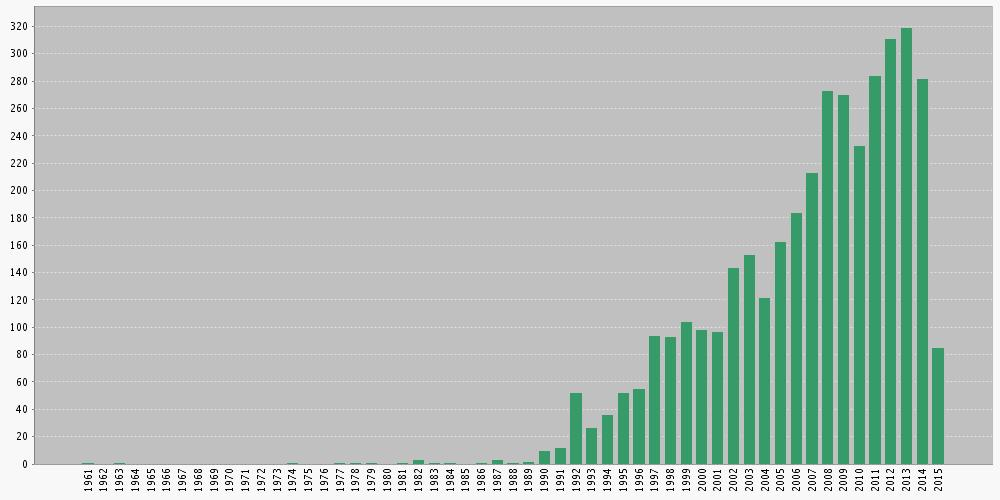
\includegraphics[scale = 0.4]{Images/bdPubsWoS.jpeg}
\end{center}
\caption{ A histogram of publications containing the keywords ``Bycatch'' or ``Discards'' found in the categories {\bf Fisheries, Biodiversity Conservation, Marine Freshwater Biology, Environmental Sciences or Ecology}. Source: Web of Science.}\label{fig:WoSPubRep}
\end{figure}

\begin{figure}[!h]
\begin{center}
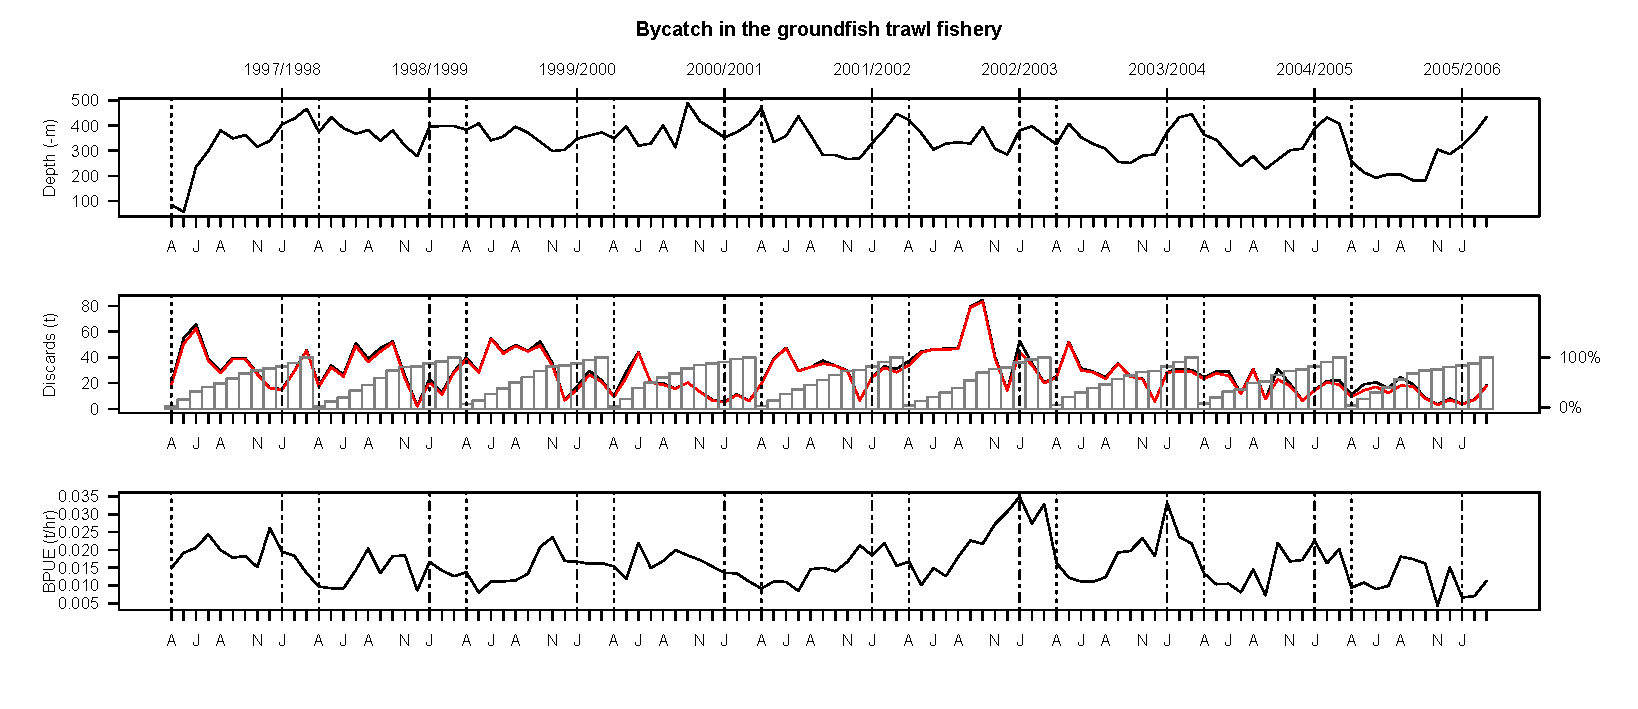
\includegraphics[scale = 0.55]{Images/ts.pdf}
\end{center}
\caption{Time series of average depth of trawling, total discards in tonnnes and bycatch per unit of effort in tonnes per hour, over the entire BC GTF between 1997 and 2006. The red line in the bycatch time series is the juvenile discarding, while the black line represents the total. The grey histogram behind the discarding time series are cumulative distributions of discarding for each year.} \label{fig:bycatchTS}
\end{figure}


\begin{figure}[!h]
\begin{center}
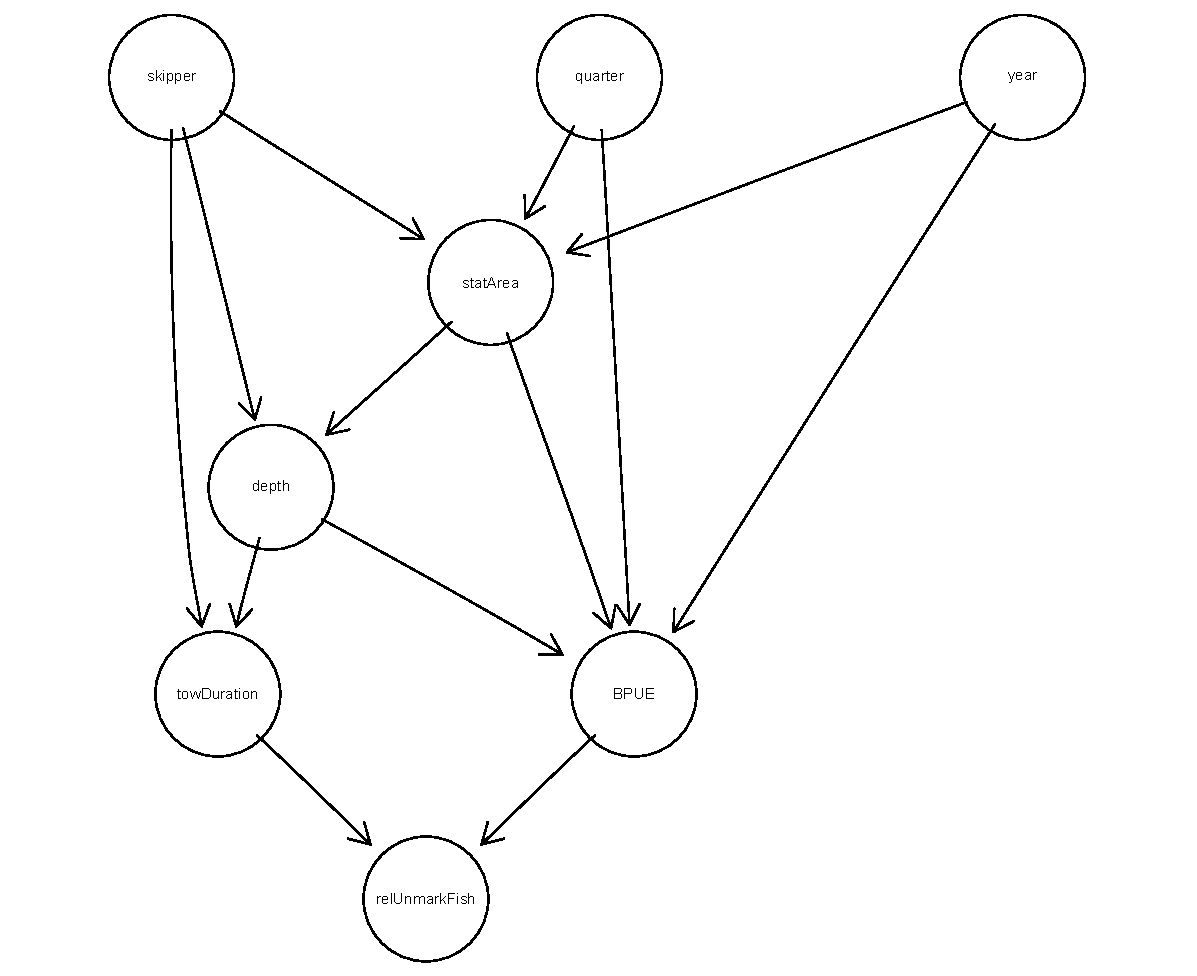
\includegraphics[scale = 0.8]{Images/BN.pdf}
\end{center}
\caption{A plot of the initial Bayesian network structure we'll be using in our attempt to predict discarding. The variable statArea corresponds to the statistical management area of the GTF; quarter is the fishing season; BPUE is the bycatch per unit of effort (t/hr); and relUnmarkFish is the tonnage of released (discarded) unmarketable fish. We believe the remaining variables to be self explanatory. } \label{fig:BN}
\end{figure}



\end{document}
     
% \begin{itemize}
%   \item Definition: removals of target and non-target species which aren't accounted for in landings.
%   \item Bycatch is commonly considered non-commercial species, such as marine mammals and other megafauna, however commercial species are also affected, usually by selective discarding like high-grading.
%   \item \citet{hall2005managing} give a review of fisheries bycatch, citing \citet{AlversonEtal1994} and \citet{kelleher2005discards}. Includes a nice summary of reduction techniques, including techological, social and legislative approaches and an agent oriented approach framework. \sj{harvest more citations from Hall and Mainprize.}
%   \item Avoidance is often gear-based (BRDs, TEDs - grates over trawl nets, circle hooks etc, mesh size) or time/space closure based \sj{Citation}
%   \item Communication also helps prevent bycatch, but regulatory framework can be stifling. \sj{Citation} - \citet{gauvin1995implementation} write about a voluntary communication program \sj{Can't get a copy of the article}
%   \item ITQs for total catch rather than landings are commonly used to encourage harvesters to avoid bycatch species. ASOPs help keep them honest, and without them high-grading can be an issue \citep{branch2004influence} \sj{Check citation here}
%   \item \citet{Abbott2009195} give an economic/game theoretic model for legislative approach of TACs for bycatch, finding that equilibrium behaviour is characterised by excessive discarding, short seasons, foregone target species catch. They also 
%   \item \citet{AlversonEtal1994} found that discard mortality accounted for 17.9 - 39.5 million metric tonnes in the late 1980s \sj{annual figure?}, computing bycatch mortality as a function of landings
%   \item \citet{kelleher2005discards} used a different methodology, computing bycatch mortality as a function of a fishery (area, gear, stock) and produced a most probably figure of around 6.8 million metric tonnes.
%   \item \citet{davies2009defining} attempt to define and estimate global fisheries bycatch. Under their methodology and definition, bycatch accounts for approximately $40\%$ of removals from marine fisheries globally.
%   \item \citet{hall2005managing} suggest that overall reductions in bycatch of between 25\% and 64\% if global fishing fleets can match min - median performance of gear modificiations in experimental studies \sj{Find reasons why gear based methods aren't being picked up - a comparison of gear based methods to data-based methods would be good for economic chapter}
%   \item Costs of bycatch - 4 categories from \citet{hall2005managing}. Also, read \citet{pascoe1997bycatch} - they estimate $\sim20\%$ of removals are discards.
%   \item Why can't we use legislative or gear-based techniques? What about social approaches?
%   \item Boundary: Bycatch avoidance schemas\sj{?} based on gear (conservation engineering \sj{citation}) are either under-adopted or reaching their maximum potential effectiveness \sj{Citation, or restatement}. Data collected by fisheries are often left dormant either before or after its intended use. There are obvious opportunities for a study of increased data and fleet communication based techniques for bycatch avoidance. \sj{Include info about agent oriented approach, why there might be low adoption}
%   \item {\bf Overview of contribution:} Major question is `How can data collection, utilisation and reutilisation be improved to facilitate the avoidance of bycatch species?'        
% \end{itemize}


% \section{A Review of Movement Ecology and Bycatch Reduction} \label{sec:MoveReview}

% \begin{itemize}
%   \item Sablefish are a highly migratory species, with habitat ranging from northern california, north along the west coast of North America and around through the Gulf of Alaska into the Bering Sea.
%   \item The life history of sablefish is rather obscure: there is information about their spawning habits, nursery habitats and coarse level migration information and little else. \sj{citations, justification}
%   \item Succesful avoidance of sablefish by the GTF will require finer detail on movement, both at the population level and at the level of smaller subgroups (schools); this will require a literature review of movement ecology.
%   \item Some selected references are given below. \sj{Take excerpts from these, or find others which are more suitable.}
%   \item Movement
%     \begin{itemize}
%       \item \citep{nathan2008movement}
%         \begin{itemize}
%           \item 
%         \end{itemize}
%       \item \citep{fryxell2008multiple}
%         \begin{itemize}
%           \item A central theme of the movement ecology framework is that of mulitple movement modes - at a fine scale, foraging vs resting.
%           \item \citet{fryxell2008multiple} confirm the existence of bi-phasic movement of introduced elk at fine (metre-minutes), intermediate (km-hours) and coarse (100's km - years) scales.
%           \item It would be interesting to see a different example on a group that wasn't introduced to an area: having coarse scale movement when introduced doesn't seem suprising to me, due to the confounding factor of unfamiliar territory.
%           \item Multi-phasic movement information is missing for Sablefish, due to low resolution tagging data.
%         \end{itemize}
%       \item \citep{pittman2003movements}
%       \item \citep{heifetz1991movement}
%       \item \citep{getz2008framework}
%         \begin{itemize}
%           \item \citet{getz2008framework} give a mathematical framework to complement the theoretical model of \citet{nathan2008movement}, which can be used to simulate or estimate (state space approach) data.
%           \item Many modern movement models assume homogeneity of fundamental movement elements (FMEs) over long time periods - for example always walking or trotting at the same pace for a given time step - due to the low resolution of time sampling for data-collection. More realistically, we can expect that animals are probably taking a ``compromise'' movement approach (or at least can't expect that they're taking a single-phase walk) - for example heading home to sleep for the night via the pub for one beer - and \citet{getz2008framework} build this into their model by considering composites of FMEs known as canonical activity modes (CAMs).
%           \item The model they introduce is very general, but includes habitat preference influences - landscape, safety, food availability etc - all things that we should include.
%         \end{itemize}
%       \item \citep{righton2008reconstructing}
%         \begin{itemize}
%           \item \citet{righton2008reconstructing} reconstruct the migration paths of groundfish by using data obtained from data-logging tags.
%           \item Data loggers are deployed similarly to normal tags and record (depth/pressure)? \sj{Is it one or both?} and temperature at a certain time resolution \sj{Check}. Tags are collected by commercial fishing efforts and returned to the researchers in exchange for a reward.
%           \item \citet{righton2008reconstructing} fit the tag data on temperature and depth to an oceanographic model to create a list of candidate locations for each timestep. Under some assumptions about fish movement rates and vertical placement (movement is along the bottom), a collection of possible paths through candidate locations is generated by simulation. A `most likely' path is chosen by using a MLE type procedure, one for each metric of `most likely' \sj{Get details from paper if necessary}.
%           \item It struck me that movement in this case was considered totally single-phase. It would be interesting to test out how using CAMs in the simulation stage might affect the possible paths - as well as the possibility of letting the fish off the bottom.
%         \end{itemize}
%     \end{itemize}
%   \item Bycatch
%     \begin{itemize}
%       \item \citep{safina2008study}
%       \item \citep{lewison2009mapping}
%       \item \citep{sims2008modeling}
%       \item \citep{hall2005managing}
%     \end{itemize}
% \end{itemize}


% \item BC Groundfish Trawl fishery
%   \begin{itemize}
%     \item Under a lot of scrutiny for bycatch of other commerical species and habitat impact (though this is quite positive now, see Scott Wallace's videos at DavidSuzuki.org)
%     \item manages 55 stock area pairs, but achieves 4 stock assessments per year.
%     \item Scott Wallace/David Suzuki Foundation give their partial thumbs up, have worked with GF trawl for many years to improve their performance
%     \item SeaChoice (an ecocertification group) gives 88\% of BC GF trawl product their approval

%   \end{itemize}

% \begin{itemize}
%   \item Groundfish fisheries in BC - Sablefish, Halibut and GTF
%   \item Sablefish are declining, is this due to bycatch in other fisheries?
%   \item Quota for every species that comes over the side, including corals and sponges.
%   \item 100\% ASOP in GTF - one of the most monitored trawl fisheries in the world. Gads of trustworthy data.
%   \item A unique opportunity to study data-based methods for improving conditions in all three areas: bycatch, habitat and sustainability
%   \item juvenile sablefish bycatch in BC GTF - unmarketable sabelfish discarding accounts for $\sim 95\%$ of discarded sablefish. The effect of discarding induced mortality on the stock is unknown.
%   \item {\it Questions:} \sj{Order these, or mention they aren't in any particular order - essentially these will correspond to chapter titles}
%     \begin{itemize}
%       \item {\it What, if any, are the predictors for the presence of non-target species?}
%       \item {\it How can we improve the spatial and temporal resolution of movement data without exploding the cost?}
%       \item {\it How can fleet communication be used to avoid non-target species? What aspects can be automated?}
%       \item {\it What general equipment can be designed to integrate the movement detection and fleet communication into a real-time feedback system to facilitate harvester avoidance of bycatch species?}
%       \item {\it What is the marginal economic benefit for avoided juvenile sablefish bycatch?} \sj{An economic analysis of the costs of discarding now, and the benefits of proposed schemes. Really investigate the reduction in target species from avoidance schemes.}
%     \end{itemize}
% \end{itemize}

% two questions in this chapter. The first is ``What are the main drivers of sablefish bycatch and discarding?''. These are currently unknown, but could either be social or ecological \citep{jannot2013identifying}. Social drivers are those determined by the harvesters themselves, such as tow duration and when and where to fish, and are most easily controlled using incentives. Ecological drivers are those determined by the habits of the species, such as habitat preference and spawning times, and are often controlled for by time-area closures.



% It is unclear into which category the drivers of sablefish discarding fall. On the one hand, migratory and breeding habits of sablefish give rise to a seasonal regularity of movement at the population level \citep{beamish1988resident}. This regularity might explain the annual pulse of increased juvenile discarding in the GTF, as shown in Figure \sj{include figure}. On the other hand, an exploratory analysis of unmarketable sablefish discarding in the GTF shows that there is a subset of skippers who are responsible for a larger proportion of discarding than might be expected. Those skippers who discard more than 1t of unmarketable sablefish in a single fishing event are responsible for around 72\% of fishing events and 82\% of the discarding. \sj{confirm} Given this slight bias in the proportion discarding, it may be that the other skippers are succesfully avoiding areas of high juvenile density.

% In this chapter we aim to identify the predictors of events with a large volume of sablefish discarding from commercial data and classify them as either ecologically or socially driven. Identification and classification of predictors will allow for formulation of possible regulatory structure to facilitate avoidance, such as time-area closures or incentive schemes, which can be later tested for their implications. Finally, we aim to provide an expected total weight of discarding per trip for given initial conditions, found by fitting a Bayesian network to historic trawl data with the identified predictor variables.


% \begin{itemize}
%   \item Bycatch rates for sablefish are high across the fished areas of the GTF and appear to have a seasonal pattern. \sj{supporting evidence from the GTF data}
%   \item Commercial fishing data contain many potential temporal, spatial and environmental predictors, which can be combined with other sources of environmental data. \sj{Sources}
%   \item We aim to identify potential predictors of sablefish density across the BC coastal GTF and build a predictive spatial model for sablefish density, collated by season (or a finer timescale, if appropriate).
%   \item Are there social/human actions at play? Are large events isolated, or did the skippers see them coming and keep fishing anyway? \sj{This is probably a different chapter}
% \end{itemize}


% \section{A movement model to estimate migration habits and local abundance.}\label{sec:MarkovMovement}

% \sj{If we're removing content, this might be the first to go.}

% \subsection{Background}
% \begin{itemize}
%   \item Nearshore inlets, which provide a nursery habitat for juvenile sablefish, have been closed to directed sablefish fishing since '94 \sj{citation}.
%   \item Inlet surveys have been tagging fish for ~20 years, giving a lot of coarse grain movement data.
%   \item It is unclear how the abundance in the inlets has changed since the closures, what the contribution of the inlets is to the directed fisheries offshore and whether or not the inlets act as a source for sablefish recruitment to the directed fisheries.
% \end{itemize}

% \subsection{Methods}

% \begin{itemize}
%   \item Existing tagging data will be used to generate movement probabilities between tagging locations and major-minor statistical areas, giving a coarse scale Markovian movement model \citep{mcgarvey2002estimating}.
%   \item The movement probabilities will be used in a Jolly-Seber type model, stratified by tagging cohort, along with survey and commercial fishery catch per unit of effort (CPUE) to provide estimates of abundance in the nearshore inlets \citep{brownie1993capture}.
% \end{itemize}

% \subsection{Expected Results} 

% \begin{itemize}
%   \item Initial exploration of the tagging data shows empirically that 21\% of the tag recoveries in offshore fisheries originate in inlet surveys.
%   \item We expect to find that the nearshore inlets do indeed provide a source of sablefish recruitment (proportion to be determined) but that the sablefish are being intercepted in either the GTF of longline fisheries while migrating during their juvenile stage.
% \end{itemize}

% \subsection{Challenges and Propsed Solutions}
% \begin{itemize}
%   \item The results could be controversial as there is a sentiment that the GTF is responsible for the decline in local sablefish abundance due to their interception of juveniles - this research could confirm the suspicions and further harm the GTFs economic competitiveness in the marketplace.
%   \item Solution: Thoroughly test this hypothesis against any and all data.
%   \item Challenge: Results could be inconclusive, possibly due to low resolution of movement data from traditional tagging experiments.
%   \item Solution: Investigate increased resolution of movement data.
% \end{itemize}

% \begin{itemize}
%   \item Tagging experiments typically provide only two data points - mark and recapture - for each indivdual, and due to reporting incentives \sj{citation} often require removal of the individual from the stock for the second point.
%   \item We estimate the required sample size for increasing movement resolution through the use of acoustic tags and detection devices deployed on fishing gear.
%   \item IDEA: partial replacement of trad tags by data loggers - if tag independence is a fantasy, can we exploit the dependence for a saving on the tagging experiment? This would require an estimate of dependence for some power analysis purposes.
% \end{itemize}

% \begin{itemize}
%   \item The required sample size is computed by way of a power analysis using a simulation model of the GTF and inlet surveys.
%   \item An individual based model with Sablefish modeled by SDEs with a habitat preference (depth) and process error and boats modeled using DEVS, where interfishing times, trip length and docking behaviour is based on historical fishing activity. SDEs allow fish paths to be generated at the beginning of the model; DEVS are used because the boats can only possibly detect when fishing gear is deployed - both of these will provide computational advantage.
%   \item Based on an estimated detection efficiency, a record of the detections of simulated fish as if they were acoustically tagged will be compared to detections through fishing mortality (traditional tagging), to check the required sample size for increased resolution of movement behaviour.
% \end{itemize}

% \begin{itemize}
%   \item \citet{hall2005managing} outline some other communication strategies - there are sometimes $\sim 50\%$ reductions in bycatch of marine mammals. \sj{citation in Mendeley.}
%   \item \citet{gauvin1995implementation} have an example of fleet communication avoidance strategies in the Bering Sea, which is revisited by \citet{gilman2006fleet}.
%   \item It's possible that this is already happening among small cliques of harvesters, but it's hard to know if it is, or if it's having any effect.
% \end{itemize}

% \begin{itemize}
%   \item Pilot analysis: individual based model of fishing behaviour in conjunction with spatial model of sablefish from previous chapter.
%   \item Move on to 
%   \item Front-end: iPads (or similar) to report bycatch incidence, direct communications to central hub
%   \item Back-end: central communications hub, receiving data from iPads, updating spatial models and rebroadcasting predictions of bycatch hotspots based on historic data (oceanography, past commercial fishing, environmental effects) and real time feedback from communcations system.
% \end{itemize}

% \begin{itemize}
%   \item expensive, hard to sell to fishers, whether to legislate/regulate?
%   \item A fleet communication program is likely an ineffective strategy to address a fishery's bycatch proble when the incidence of interactions with the bycatch species is a common event and occurs across the fleet's fishing grounds, and in fisheries where there is a lack of economic incentives to reduce bycatch \citep{gilman2006fleet}
%   \item A bottom up approach of developing the fleet communications with harvesters. 
%   \item Might require some economic analysis to show future benefits outweigh costs, al la \citet{gilman2006fleet}
%   \item Pilot experiment to show benefits with a control group and a treatment group of boats.
% \end{itemize}

% \begin{itemize}
%   \item Data should be used at least twice.
%   \item With the right resolution on data, sustainability can be improved with low cost.
%   \item There are diminishing returns on sustainabile engineering (gear based bycatch reduction) - data based methods can (hopefully) be used as a substitute
%   \item Talk about how this might be applied elsewhere, in data limited situations, or be used as an argument for improving data resolution in those areas
%   \item Future work
% \end{itemize}
